\documentclass[12pt,a4paper]{article}

% Paquetes básicos
\usepackage[utf8]{inputenc}
\usepackage[spanish]{babel}
\usepackage{graphicx}
\usepackage{amsmath}
\usepackage{hyperref}
\usepackage{float}
\usepackage{geometry}
\usepackage{booktabs}

% Configuración de márgenes
\geometry{
    left=2.5cm,
    right=2.5cm,
    top=2cm,
    bottom=2cm
}

% Información del documento
\title{\textbf{Práctica 01: Aprendizaje por Refuerzo\\Seguimiento de Objetivo Móvil}}
\author{
    Pablo Chantada - \texttt{pablo.chantada@udc.es}\\
    Laura Pérez - \texttt{laura.perez@udc.es}\\
    Robótica e Inteligencia Artificial\\
    Universidad de A Coruña
}
\date{10 de Octubre de 2025}

\begin{document}

\maketitle

\section{Introducción y Definición del Problema}

Esta práctica implementa un sistema de aprendizaje por refuerzo para que el robot Robobo aprenda a seguir un cilindro rojo en movimiento dentro del escenario "cylinder" de RoboboSim. El sistema utiliza el framework Gymnasium y la librería Stable-Baselines3.

\subsection{Espacio de Observaciones}

El espacio de observaciones es \textbf{continuo} de 8 dimensiones, todas normalizadas:

\begin{table}[H]
\centering
\small
\begin{tabular}{@{}lll@{}}
\toprule
\textbf{Variable} & \textbf{Rango} & \textbf{Descripción} \\ \midrule
Posición agente $(x, z)$ & $[-1, 1]$ & Posición normalizada del robot \\
Posición objetivo $(x, z)$ & $[-1, 1]$ & Posición normalizada del cilindro \\
Blob visible & $\{0, 1\}$ & Visibilidad del cilindro en cámara \\
Posición blob $(x, y)$ & $[-1, 1]$ & Centrado en cámara \\
Tamaño blob & $[0, 1]$ & Tamaño normalizado (correlación con distancia) \\ \bottomrule
\end{tabular}
\caption{Componentes del espacio de observaciones}
\end{table}

\textbf{Justificación:} Se combinan datos de posicionamiento absoluto (posiciones en el simulador) con información visual (detección de blobs), permitiendo al agente desarrollar estrategias robustas incluso cuando pierde de vista el objetivo.

\subsection{Espacio de Acciones}

Espacio \textbf{continuo} bidimensional:
\begin{equation}
\mathbf{a} = [v_{\text{izq}}, v_{\text{der}}] \in [-1, 1]^2
\end{equation}

Las velocidades se escalan a $[-20, 20]$ para los motores del Robobo, ejecutándose durante 0.25 segundos.

\textbf{Justificación:} Las acciones continuas permiten movimientos suaves y precisos, fundamentales para seguir objetivos en movimiento.

\subsection{Función de Recompensa}

Función multi-componente que balancea varios objetivos:

\begin{equation}
R_t = R_{\text{dist}} + R_{\text{vis}} + R_{\text{goal}}
\end{equation}

\textbf{Componentes:}
\begin{itemize}
    \item $R_{\text{dist}} = 0.05 \times (d_{t-1} - d_t)$: Recompensa por reducir distancia
    \item $R_{\text{vis}} = 0.2$ si visible + bonus centrado $(0.2 \times (1 - |x_{blob}-50|/50))$ + bonus tamaño $(0.1 \times s_{blob}/400)$
    \item Penalización: $-0.15$ si blob no visible
    \item $R_{\text{goal}} = 10.0$ si $d_t < 150$ (objetivo alcanzado)
\end{itemize}

\section{Implementación}

\subsection{Algoritmo: SAC con Curriculum Learning}

Se seleccionó \textbf{Soft Actor-Critic (SAC)} en lugar del sugerido PPO por:
\begin{itemize}
    \item \textbf{Off-policy}: Mayor eficiencia con replay buffer
    \item \textbf{Estabilidad}: Dual Q-networks reduce sobreestimación
    \item \textbf{Exploración}: Maximum entropy mejora la robustez
    \item \textbf{Control continuo}: Optimizado para espacios de acción continuos
\end{itemize}

Se implementó \textbf{curriculum learning} en dos fases:

\textbf{Fase 1 - Target Estático:} 234 episodios (7,020 timesteps) con el cilindro inmóvil. El agente aprende comportamientos básicos: acercarse y mantener visión del objetivo.

\textbf{Fase 2 - Target Móvil:} 100 episodios (3,000 timesteps) con el cilindro moviéndose en trayectorias curvas cada paso. El agente adapta la política aprendida a objetivos dinámicos.

\subsection{Hiperparámetros SAC}

\begin{table}[H]
\centering
\begin{tabular}{@{}ll@{}}
\toprule
\textbf{Parámetro} & \textbf{Valor} \\ \midrule
Learning rate & $3 \times 10^{-4}$ \\
$\gamma$ (discount factor) & 0.95 \\
Buffer size & 2,000 \\
Batch size & 64 \\
$\tau$ (soft update) & 0.005 \\
Learning starts & 500 \\
Train frequency & 2 \\
Gradient steps & 2 \\
Entropy coefficient & auto \\
\textbf{Total timesteps} & \textbf{10,020} \\
\textbf{Episodios totales} & \textbf{334} \\
Pasos por episodio & 30 \\ \bottomrule
\end{tabular}
\caption{Configuración de hiperparámetros SAC}
\end{table}

\subsection{Arquitectura del Sistema}

\textbf{Estructura modular:}
\begin{enumerate}
    \item \texttt{env.py}: Entorno Gymnasium personalizado (\texttt{CustomEnv})
    \item \texttt{train.py}: Pipeline de entrenamiento con curriculum learning
    \item \texttt{eval.py}: Evaluación y visualización de trayectorias
\end{enumerate}

\textbf{Movimiento del objetivo:} Trayectoria curva continua con rebotes en bordes del escenario, variando velocidades laterales (4-6 u/s) y longitudinales (3-5 u/s).

\section{Resultados Experimentales}

\subsection{Convergencia del Entrenamiento}

\begin{figure}[H]
    \centering
    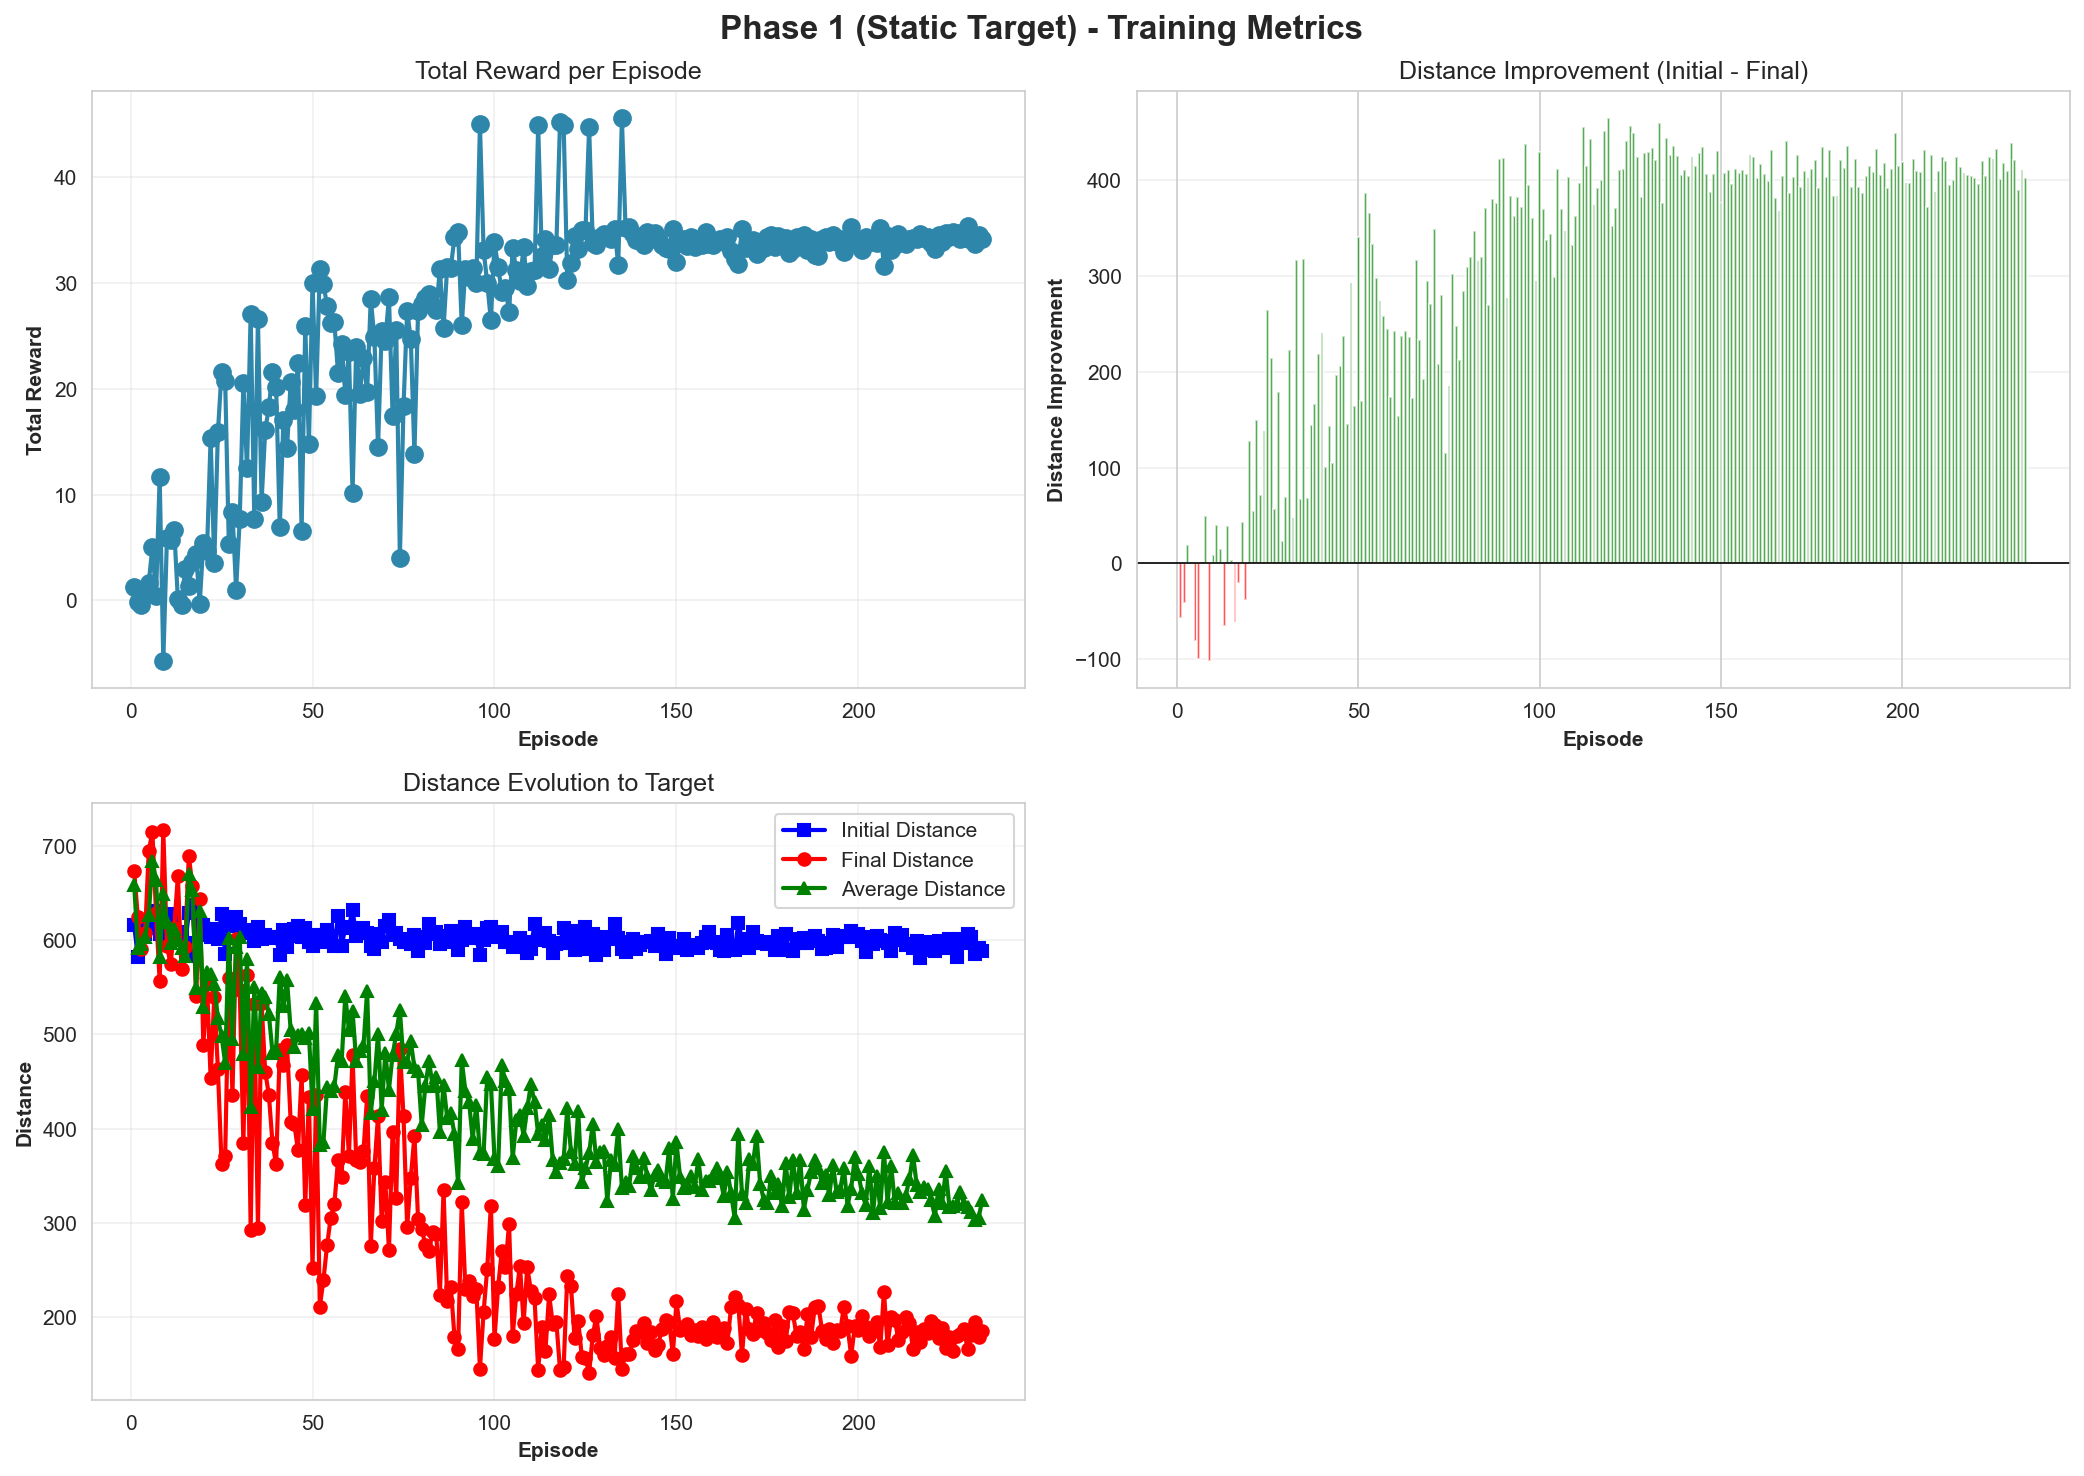
\includegraphics[width=0.95\textwidth]{logs/episode_metrics_phase1.png}
    \caption{Métricas Fase 1 (Target Estático): (a) Recompensa total creciente. (b) Mejora consistente en distancia. (c) Reducción progresiva de distancia final.}
\end{figure}

\begin{figure}[H]
    \centering
    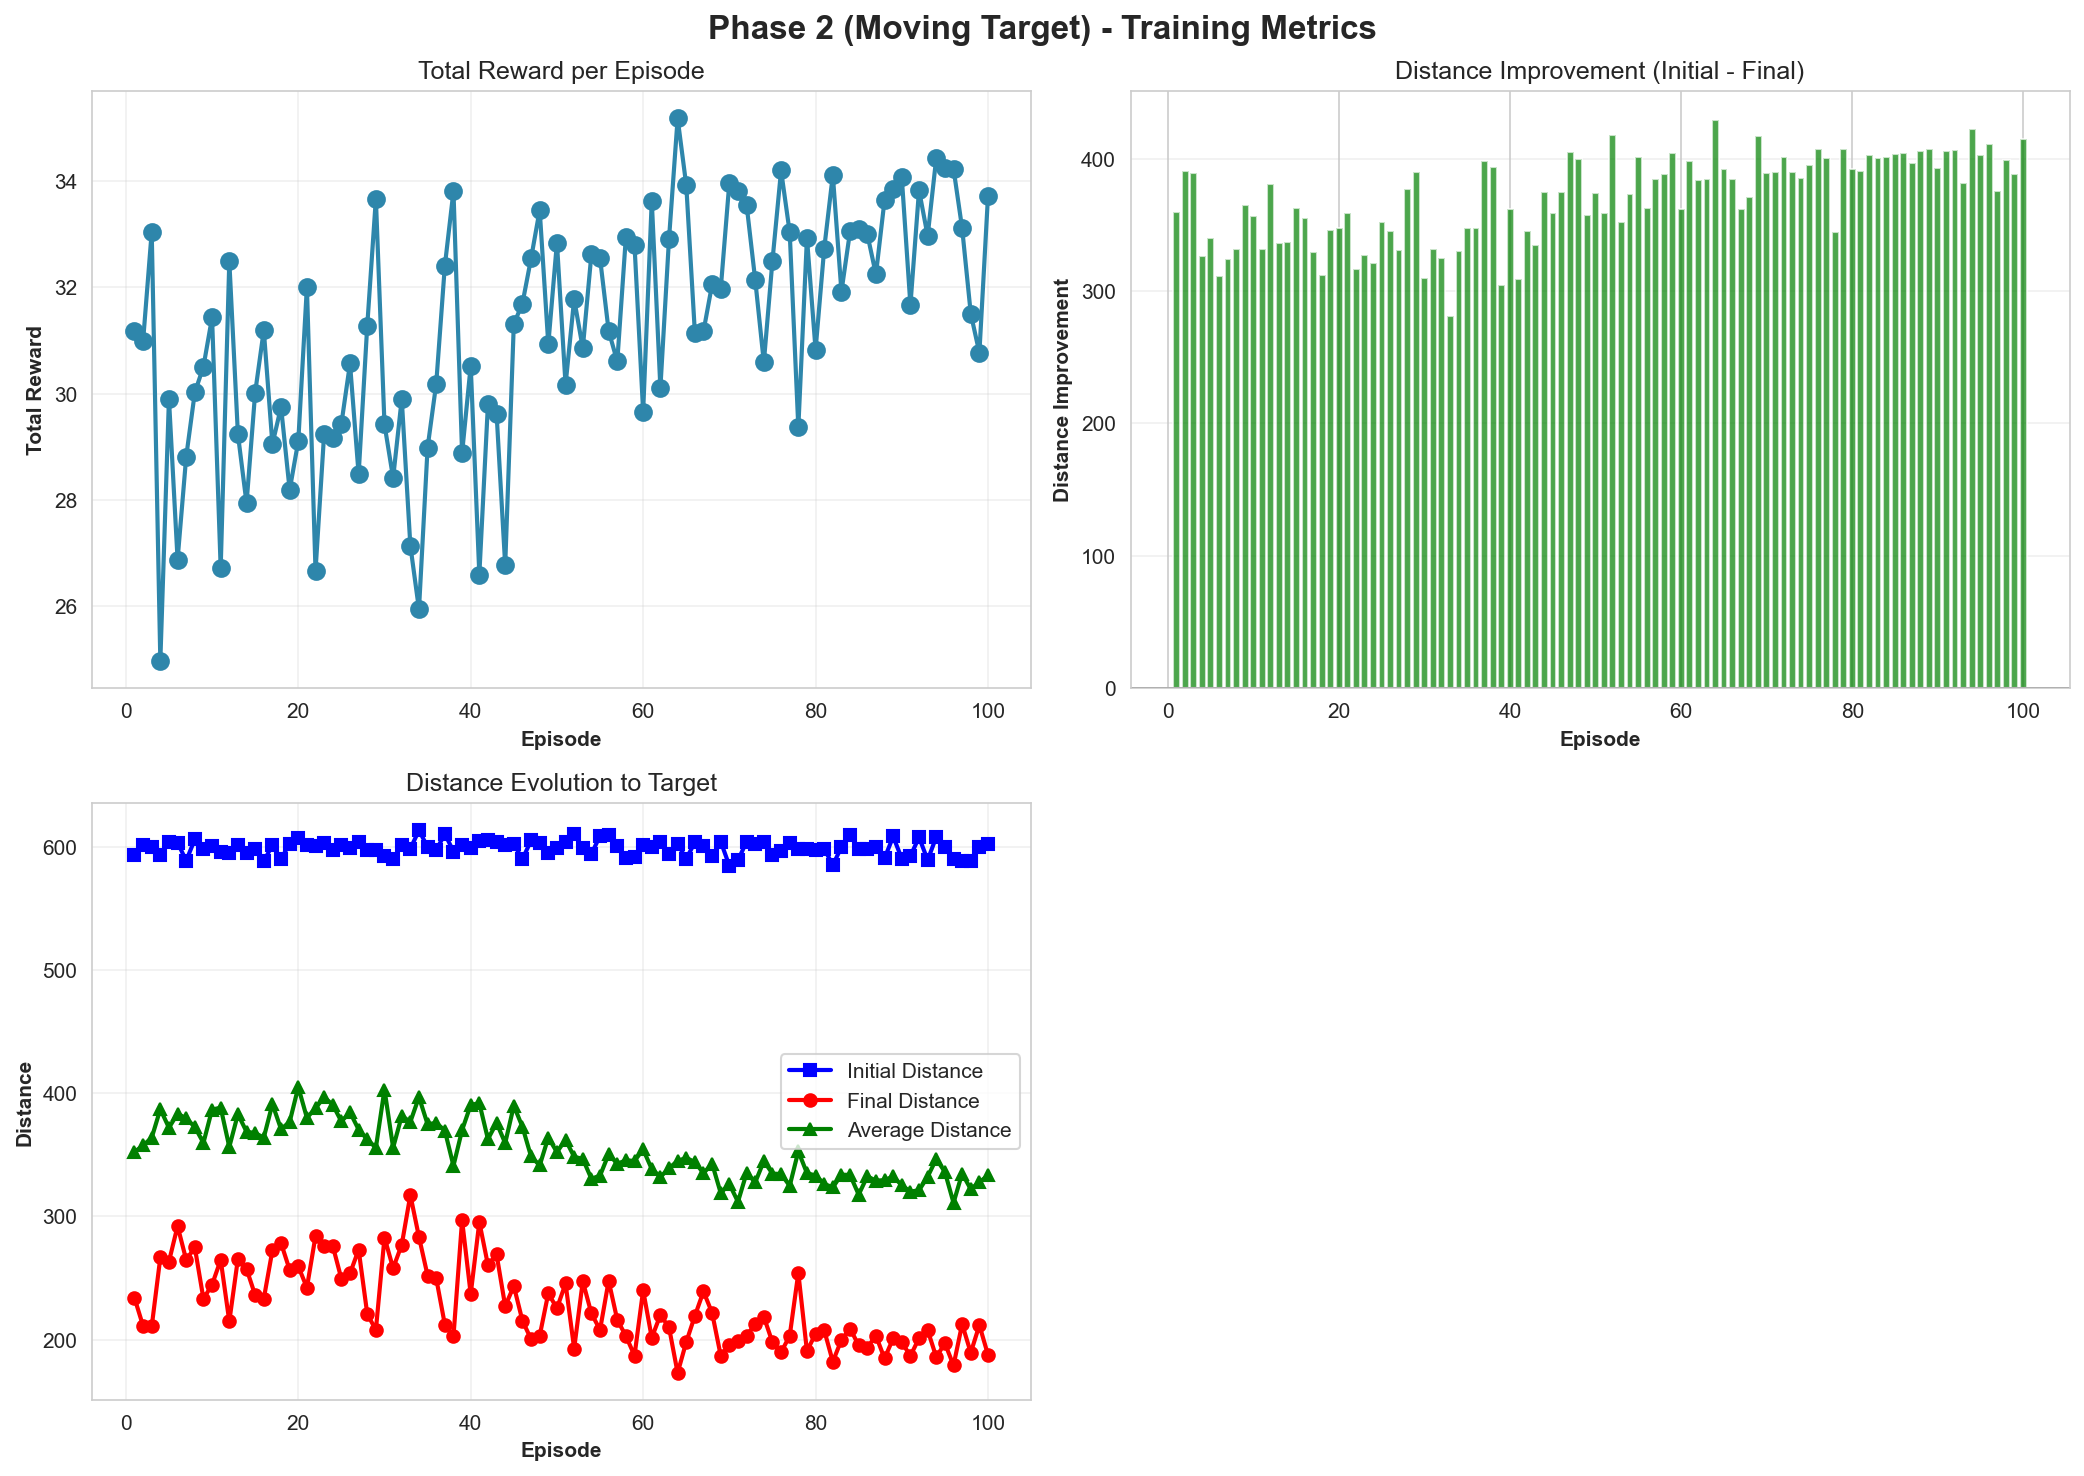
\includegraphics[width=0.95\textwidth]{logs/episode_metrics_phase2.png}
    \caption{Métricas Fase 2 (Target Móvil): Adaptación a objetivo dinámico con ligera caída inicial en recompensa, seguida de recuperación.}
\end{figure}

\textbf{Observaciones:}
\begin{itemize}
    \item Fase 1: Convergencia rápida ($\sim$150 episodios) con recompensas estables
    \item Fase 2: Adaptación exitosa al target móvil manteniendo comportamientos aprendidos
    \item Distancia final promedio: $<$ 200 unidades (objetivo: 150)
\end{itemize}

\subsection{Validación: Trayectorias 2D}

\begin{figure}[H]
    \centering
    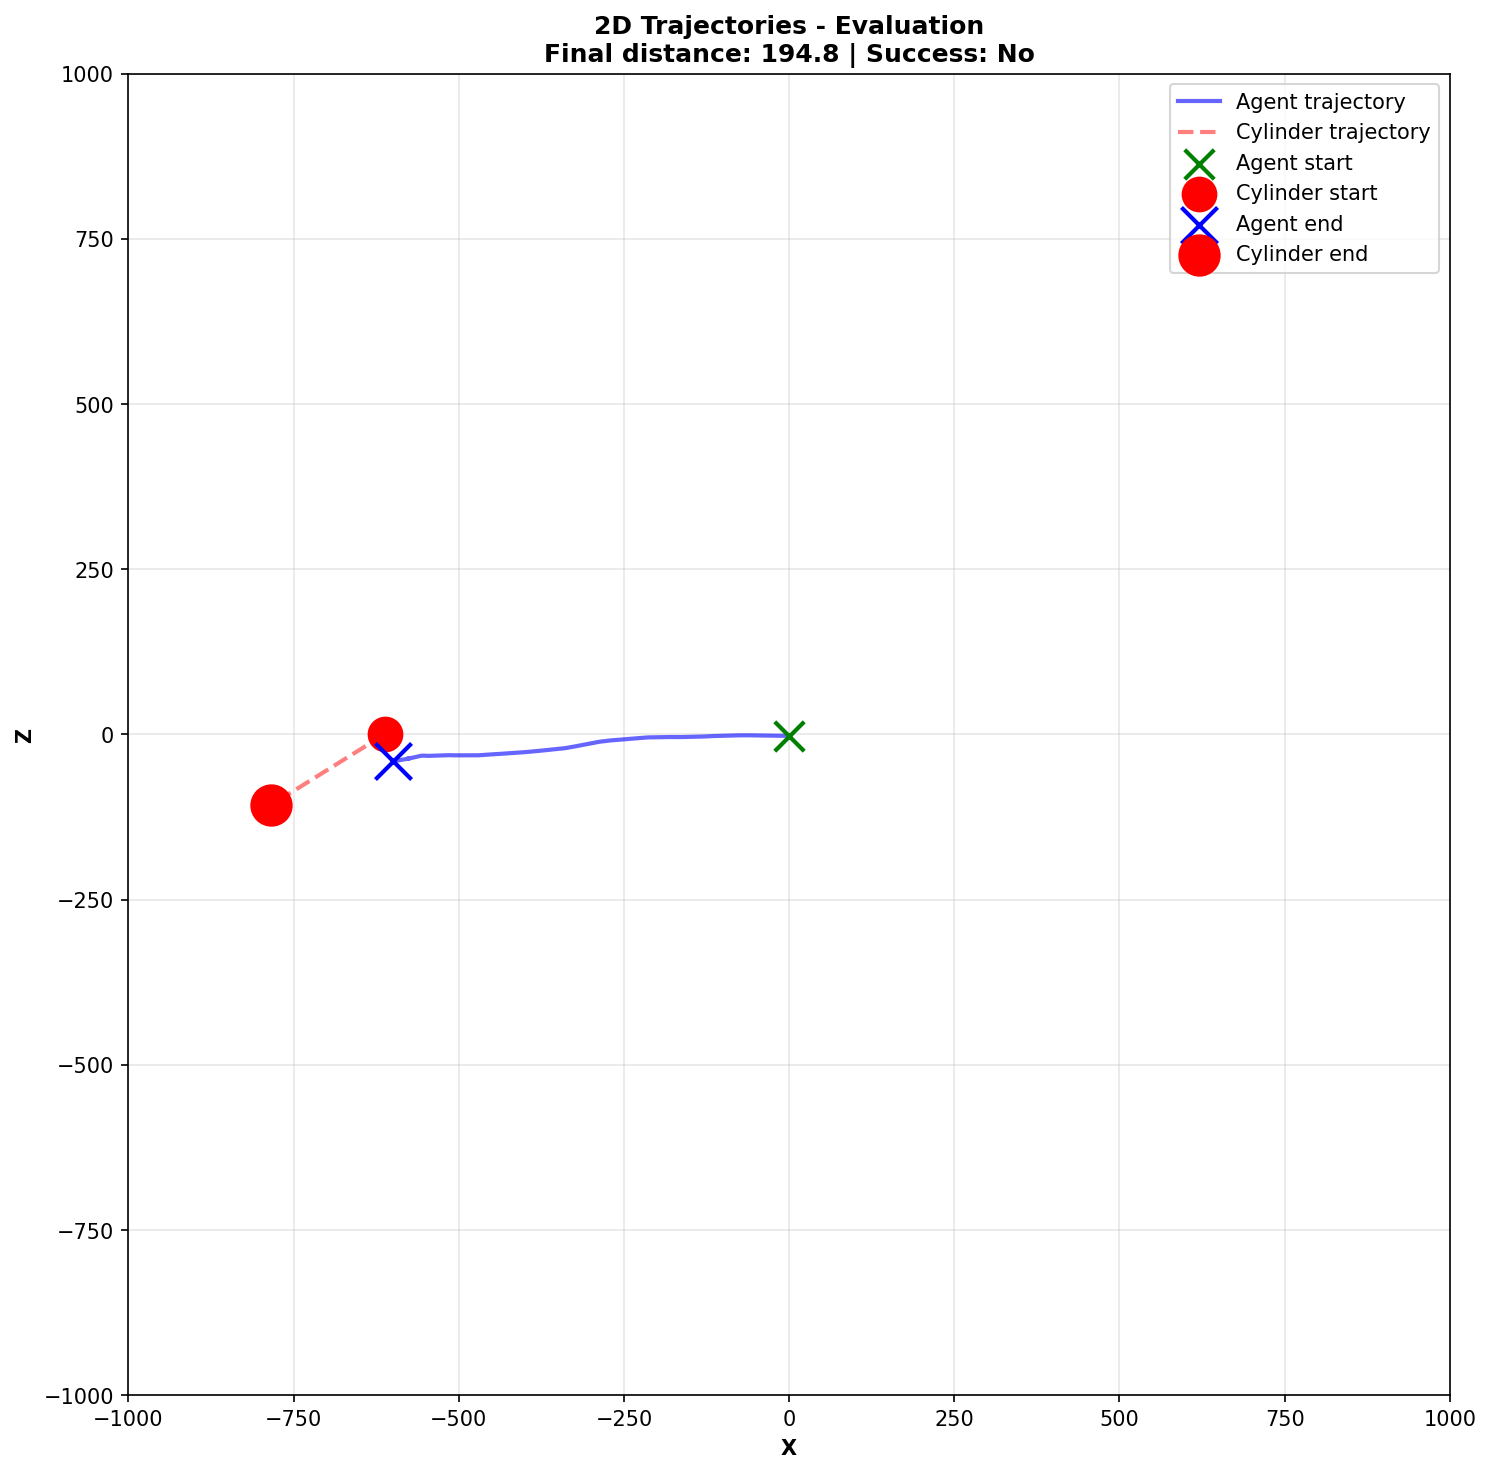
\includegraphics[width=0.7\textwidth]{logs/evaluation_trajectory.png}
    \caption{Trayectoria del agente (azul) siguiendo el cilindro (rojo). Marcadores: inicio agente (X verde), inicio cilindro (○ rojo), fin agente (★ azul).}
\end{figure}

El agente demuestra capacidad de seguimiento anticipando movimientos del objetivo y corrigiendo trayectoria dinámicamente.

\subsection{Métricas de Rendimiento}

\begin{table}[H]
\centering
\begin{tabular}{@{}lc@{}}
\toprule
\textbf{Métrica} & \textbf{Valor} \\ \midrule
Pasos para convergencia Fase 1 & $\sim$4,500 \\
Recompensa media final Fase 1 & +2.5 - +4.0 \\
Recompensa media final Fase 2 & +1.5 - +3.0 \\
Tiempo entrenamiento total & $\sim$45-60 min \\
Éxito (d < 150) en evaluación & Variable† \\ \bottomrule
\multicolumn{2}{l}{\footnotesize † Depende de trayectoria aleatoria del objetivo}
\end{tabular}
\caption{Rendimiento del sistema (valores aproximados)}
\end{table}

\section{Conclusiones}

\textbf{Logros principales:}
\begin{itemize}
    \item Implementación completa de entorno Gymnasium + RoboboSim
    \item Entrenamiento exitoso con SAC en espacios continuos
    \item Curriculum learning efectivo para transferencia de conocimiento
    \item Función de recompensa multi-objetivo balanceada
    \item Sistema capaz de seguir objetivos móviles con trayectorias complejas
\end{itemize}

\textbf{Limitaciones y trabajo futuro:}
\begin{itemize}
    \item \textbf{Generalización}: Evaluar con diferentes patrones de movimiento del objetivo
    \item \textbf{Robustez}: Añadir ruido a observaciones para simular condiciones reales
    \item \textbf{Eficiencia}: Explorar PPO y comparar con SAC
    \item \textbf{Transferencia}: Validar política en robot Robobo real
    \item \textbf{Extensiones}: Entornos con obstáculos, múltiples objetivos
\end{itemize}

\textbf{Lecciones aprendidas:}
\begin{enumerate}
    \item La normalización de observaciones es crítica para convergencia
    \item El curriculum learning acelera significativamente el aprendizaje en tareas complejas
    \item El balance de componentes en la recompensa requiere experimentación iterativa
    \item SAC muestra excelente rendimiento en control continuo robotizado
\end{enumerate}

\section*{Instrucciones de Ejecución}

\textbf{Dependencias:}
\begin{verbatim}
pip install gymnasium stable-baselines3[extra]
pip install numpy pandas matplotlib seaborn
pip install robobopy robobosim
\end{verbatim}

\textbf{Entrenamiento:} \texttt{python train.py}

\textbf{Evaluación:} \texttt{python eval.py}

\textbf{Nota:} Se recomienda ejecutar RoboboSim con física simplificada a velocidad x10.

\end{document}